\section{Design}
I decided to code in \textit{Python} with the external library \textit{OpenCV} for simplicity.
Since I do not use the bounding boxes in the affwild dataset, the first thing I need to get is a correspondence between landmark points and the  valence for each frame of each video, the execution took almost 21 hours so I made possible to save the results as text files.

Each valence ranges from -1 to 1 and values ranging between $-0.5$  and $0.5$ were discarded, it has been done to reduce noise and rule out uncertain valences; in the end were extracted 136909 landmark-valence tuples.
Is possible for a single frame to contain more than one face as seen in figure \ref{fig:double_face} \footnote{I find bounding boxes less invasive, in this case landmark detects two faces as well.}.
Since the affwild dataset collects videos with foreground faces is reasonable to assume that the face we're interested in is the widest one, hence I pick the landmark feature with the largest euclidean distance between the first and last point (respectively the lateral commissure of the viewer's left eye and the lower lip).

\begin{figure}[h!t]
    \centering
    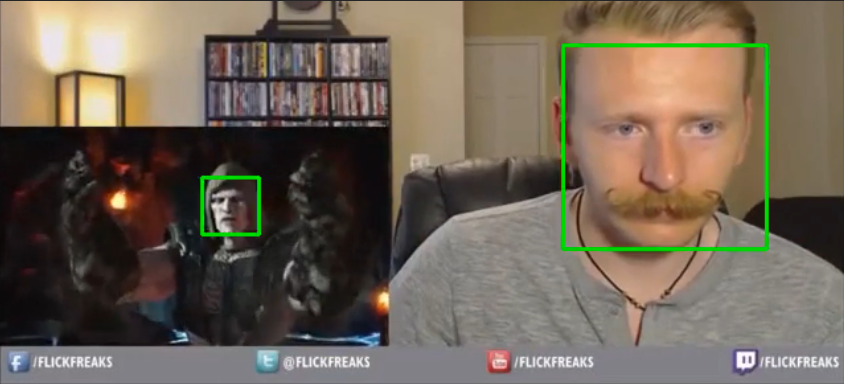
\includegraphics[scale=0.4]{images/309mp4_double_face.png}
    \caption{Two faces detected in the video 309.}
    \label{fig:double_face}
\end{figure}

Valences are saved and read as an array of floats while landmarks are a two dimensional array. 
For each face dlib stores landmark points as an array of $[x,y]$ coordinates, to make things more readable (and possibily to make the code faster in corner cases due to caching) I decided to flatten it as a one dimensional vector.
This different encoding should not change SVM's predictions.

Regarding SVM classification I first used both the OpenCV implementation and the \textit{scikit-learn} one, the latter is way better than the first and for this reason the demo uses the scikit-learn SVM.
During tests the dataset has been splitted as 80-20 percent for train and test respectively, it comes without saying that demo's SVM classifier is trained over the whole dataset.  

As said before in the demo instead of directly detecting landmark points I first detected bboxes. 
This may be odd but I noticed how given an arbitrary frame there is more probability to detect a face with dlib's landmarks than with OpenCV's haar cascade, detecting less landmarks makes the demo less precise but also makes the video smoother for a presentation.
Were used pretrained models both for bounding boxes ~\cite{dataset:haar} and landmark points ~\cite{dataset:landmark}.

The structure of classes and packages can be seen in the diagram in figure \ref{fig:packages_diagram}, it is all original code except the function \textcode{src.test.Test.plot\_roc} used to plot ROC curves. It has been taken from ~\cite{roc} as commented in the source code.

\begin{figure}[h!t]
    \centering
    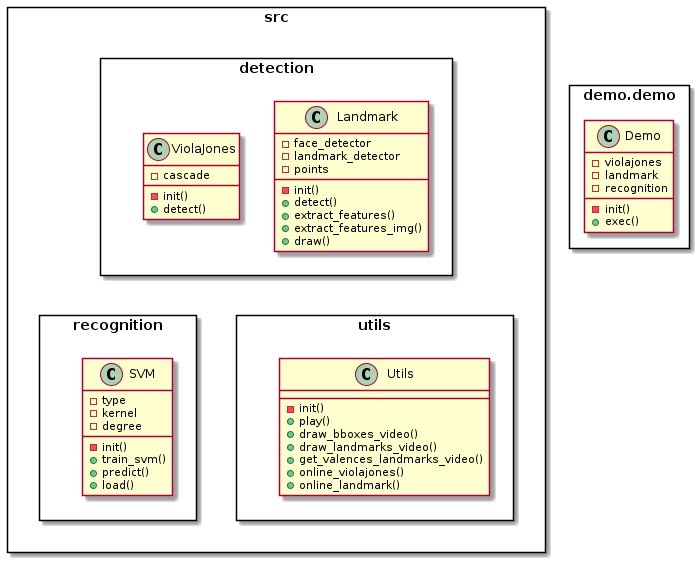
\includegraphics[scale=0.49]{../diagrams/out/classes/classes.png}
    \caption{Diagram of the packages.}
    \label{fig:packages_diagram}
\end{figure}

Other code that is not original are clearly external functions, see table \ref{tab:libraries}

\begin{table}[h!t]
    \centering
    \caption{Imported libraries}
    \label{tab:libraries}
    \begin{tabular}{ll}
        \textbf{os} & To explore the filesystem. \\
        \textbf{re} & For regular expressions. \\
        \textbf{fire} & To implement command line arguments. \\
        \textbf{numpy} & Arrays are essential thanks to the faster C implementation. \\
        \textbf{cv2} & OpenCV, used for detection with Haar features and SVM. \\
        \textbf{dlib} & In Python OpenCV landmark detection is not implemented. \\
        \textbf{sklearn} & Scikit-learn implements a more efficient SVM classifier. \\
        \textbf{joblib} & Used to save scikit-learn's SVM model. \\
    \end{tabular}
\end{table}
